\chapter{Tagging--Systeme}

\section{Grundlagen}

\subsection{Architektur von Tagging--Systemen}

\subsection{Datenmodell von Tagging--Systemen}

\subsection{Arten von Tagging--Systemen}

\section{Tagging--System von Spreadshirt}

\subsection{Spreadshirt}
\label{spreadshirt}

Die vorliegende Masterarbeit wurde im Kontext der sprd.net AG (Spreadshirt) \cite{sprd2013} erstellt. Spreadshirt ist eine E--Commerce--Plattform, die es seinen Benutzern erlaubt, personalisierte Textilien und andere Artikel zu gestalten, zu kaufen und zum Verkauf anzubieten. Spreadshirt übernimmt die Produktion und den Versand der Produkte. Ein Produkt bezeichnet hierbei einen Produkttyp, beispielsweise ein T--Shirt, der mit einem oder mehreren Designs bedruckt wurde.

Das Erstellen von Designs und die Konfiguration eines Produktes, also das Positionieren von Designs auf Produkttypen, wird vollständig vom Benutzer durchgeführt. Es agieren grundsätzlich zwei Arten von Benutzern mit der Spreadshirt--Plattform: \emph{Kunden} und \emph{Partner}.

Als Kunden werden Benutzer bezeichnet, die Produkte bestellen. Diese Produkte können entweder von ihnen selbst oder von einem Partner erstellt worden sein. 

Partner sind Benutzer, die Designs oder Produkte erstellen und diese zum Verkauf anbieten. Zu diesem Zweck kann der Partner einen eigenen Shop auf der Spreadshirt--Plattform eröffnen. Kunden können in diesem Shop Produkte bestellen und der Partner erhält einen Anteil des Verkaufspreises, während Spreadshirt die Produktion und den Versand an den Kunden übernimmt.

Neben den von Kunden für sich selbst erstellten Produkten und den Partner--Shops existiert mit dem Spreadshirt--Marktplatz ein weiterer Vertriebskanal. Auf dem Marktplatz können Partner nach ihrer Zustimmung ihre Designs vertreiben. Kunden können nach Motiven suchen, die ihrem Geschmack entsprechen und diese bestellen, mit anderen Motiven kombinieren oder mit Texten versehen. Ein Produkt, das entweder in einem Partner--Shop oder auf dem Marktplatz positioniert und mit einem Preis versehen wurde, wird Artikel genannt.

\begin{figure}
\centering
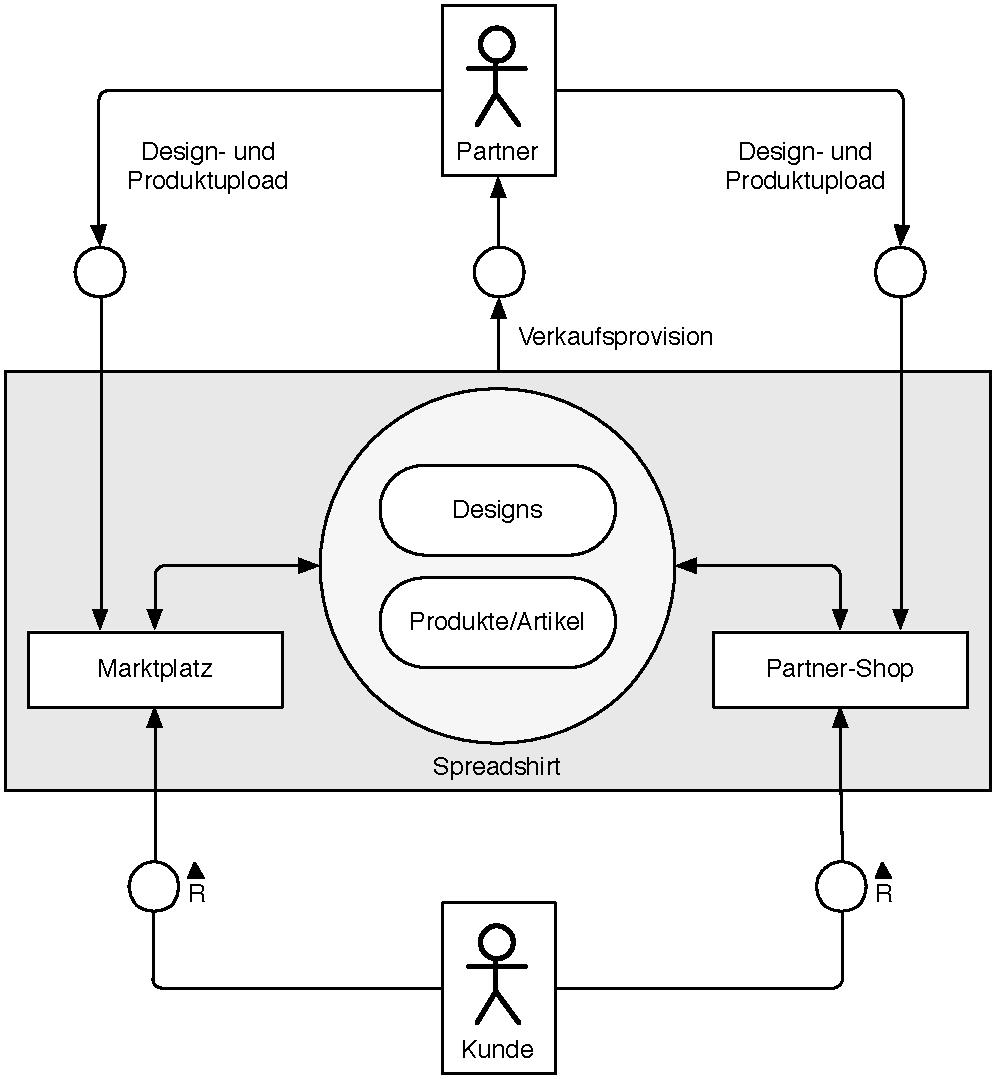
\includegraphics[width=0.7\textwidth]{how_spreadshirt_works}
\caption{FMC--Blockdiagramm der Spreadshirt--Bereiche und Benutzer}
\label{fig:howspreadshirtworks}
\end{figure}

Die grundsätzliche Funktionsweise der Spreadshirt--Plattform ist in \cref{fig:howspreadshirtworks} als FMC--Blockdiagramm dargestellt.

Das Suchergebnis für Suchen auf dem Marktplatz hängt maßgeblich von den Metadaten ab, die der Partner für seine Designs vergeben hat. Dazu gehören Tags, aber auch Titel und Beschreibung des Designs oder Produktes. In dieser Arbeit wird ausschließlich das Tagging--System betrachtet.

\label{platforms}
Spreadshirt betreibt aus historischen Gründen zwei Plattformen, deren Datenbestände größtenteils voneinander getrennt sind. Jeweils eine Plattform ist für den nordamerikanischen und den europäischen Markt zuständig. Im Kontext dieser Arbeit wird die europäische Plattform als Ausgangsbasis für alle Betrachtungen gewählt. Der Datenbestand dieser Plattform besteht aus circa 2 Millionen Tags, 6 Millionen Designs, 14 Millionen Produkten, 6 Millionen registrierten Nutzern und \num{750000} eröffneten Partner--Shops.

\subsection{Einschränkungen des Tagging--Systems}

\subsection{Datenqualität des Tagging--Systems}
\label{quality}

Die Qualität von Daten wird im Allgemeinen unter mehreren Gesichtspunkten beurteilt. Dazu gehören unter anderem \emph{Korrektheit}, \emph{Vollständigkeit}, und \emph{Redundanzfreiheit} \cite[S. 84 f.]{hkp2012}. Nachfolgend werden die bei Spreadshirt vorhandenen Tagging--Daten nach diesen Kriterien betrachtet und die Quellen eventueller Fehler \cite[S. 43 f.]{jo2003} diskutiert.

\subsubsection{Korrektheit}

Die Korrektheit der Tagging--Daten kann an vielen Punkten angezweifelt werden. Das hervorstechende Problem hierbei ist das Auftreten von Spam. Viele Partner versehen ihre Artikel und Designs mit Tags, die nicht den Inhalt beschreiben. Partner versehen ihre Designs und Artikel mit falschen Tags, damit diese bei populären Suchbegriffen gefunden werden.

Ein weiterer Defekt ist die Inkorrektheit des Attributes \emph{Sprache} der Tags. Die Sprache wird aus der Domain abgeleitet, die der Benutzer, der den Tag eingegeben hat, besucht hat. Viele Partner geben jedoch ihre Tags in mehreren Sprachen ein, um ihre Inhalte besser auffindbar zu machen. Dies führt in der Konsequenz dazu, dass das Attribut Sprache in einem nicht unwesentlichen Teil der Tags als falsch angesehen werden kann.

Die Quelle beider Fehler ist also die bewusste Falscheingabe von Informationen, um einen persönlichen Vorteil zu erlangen, da die Partner versuchen, ihre Produkte möglichst zu vielen Sucheingaben in den Ergebnissen auftauchen zu lassen.
                                                                                                                                                                                                                                                                                                                                                                                                              
\subsubsection{Vollständigkeit}

Wie bereits in \cref{tag-system} beschrieben, fehlen in den Daten des Spreadshirt--Systems der Zeitpunkt und der Benutzer eines Taggings. Dies führt in der Konsequenz dazu, dass Spam schwerer erkannt werden kann. Zwar ist bekannt, wann ein Tag das erste Mal verwendet wurde, alle weiteren Verwendungen des Tags haben jedoch keinen Zeitstempel. Der Benutzer, der den Tag angelegt und verwendet hat, kann nur daraus abgeleitet werden, wer den getaggten Artikel angelegt hat.

Die Unvollständigkeit der Daten rührt in erster Linie daher, dass zum Zeitpunkt der Implementierung des Tagging--Systems noch nicht bedacht wurde, dass die fehlenden Attribute später nützlich sein können.

\subsubsection{Redundanzfreiheit}

Bedingt durch die Form der Dateneingabe besteht für das Vokabular des Tag--Systems ein großes Potential für redundante Daten. Da eingegebene Tags durch einen Separator getrennt eingegeben werden müssen, besteht hier Potential zur Fehleingabe. Wird der falsche Separator verwendet, werden die eigentlich getrennten Tags als eine einzige Entität abgespeichert.

Technisch kann jeder Tag genau ein Mal in der Datenbank vorkommen. Jedoch führen Tipp-- und Rechtschereibfehler, unterschiedliche Groß- und Kleinschreibung, verschiedene Arten zusammengesetzte Wörter zu schreiben, Leerräume vor, nach und zwischen Wörtern eines Tags und Tippfehler dazu, dass das gleiche Wort mehrfach in der Datenbank gespeichert wurde.

Außerdem führten in der Vergangenheit Systemfehler und Implementierungsfehler dazu, dass falsche, nicht druckbare Zeichen in den Tags enthalten waren. Nach Beseitigung der Fehler blieben die fehlerhaften Tags bestehen, so dass bei einer erneuten Eingabe des gleichen Wortes ein neuer Tag in der Datenbank angelegt wurde.

\subsection{Mengengerüst}

\section{Zusammenfassung}